\chapter{Firewall and Network Security}

Protecting information can be more complex than protecting phyisical goods.
We may be interested in preventing that information can be duplicated or read by third parties.
We may wand to also protect information from being modified or erased.

The internet makes it possible for the information to easily travel accross the globe.
All the protocols and tools that are typically used with good intentions can also be used to abuse and exploit information systems.
Therefore, it is important to keep security in mind when designing and managing information networks.

Security can be present at different layers of the protocol stack.
For example, the TLS protocol offers security at the application layer in the Internet protocol stack.
TLS is used to protect HTTP sessions in the HTTPS protocol. 
The open source implementation of TSL OpenSSL was recently in the news after the heartbleed bug was discovered.

IPSEC offers security at the network layer.
It can be used to protect all traffic between two endpoints.
These endpoints can be either a host or a network.
IPsec uses two different headers to provide security.
The Authentication Header (AH) provides integrity, data origin authentication and protection against replay attacks.
The Encapsulating Security Payload (ESP) header provides confidentiality, data origin authentication, integrity and protection against replay attacks.

IPsec can operate in two diffrent modes: transport mode and tunnel mode.
In the first one, the payload of an IP packet is protected while the IP headers are left unmodified.
Even though the source and destination address are left untouched, they are still protected by a hash and therefore cannot be modified by the intermediate network devices (e.g. NAT devices).

In the second mode of operation, IPsec tunnel mode, the entire IP packet is protected and encapsulated within a new IP packet.
This tunnel can be used to create a VPN and the resulting data flow can traverse NAT devices.

Another aspect of security is access control and network perimeter protection.
It is desired to prevent unauthorized access to computers and networking devices.
In the internet there are automatized tools that are continuously looking for vulnerabilities to gain unauthorized access to systems.
Botnets are hordes of infected computers (also called zombies) that follow the commands of a master and can be used to send spam, perform port scans, or search for vulnerable systems.

Keeping the software updated and using strong passwords helps in keeping systems secure.
Another tool that helps in protecting networks and computers are firewalls.
Firewalls filter traffic and stop undesired and potentially malicious packets.
The firewall can be installed in an end computer, to protect only that computer, or in a networking device to protect a network.
We will be focusing on the latter kind of firewall.

\section{Firewall}

A network can be protected from attacks coming from the rest of the Internet by placing a firewall in the frontier between the two networks.
To be effective, it is important that all the traffic exchanged bay the network and the rest of the Internet goes through the firewall.
The firewall filters undesired traffic to offer partial protection against external attacks.
Note that a negative aspect of forcing that all the traffic between our network and the Internet is handled by the firewall is that it introduces a single point of failure.
It is possible to have two firewalls with the same configuration to mitigate this problem.

In perimeter protection, networks are called security domains and are classified regarding their level of trust.
For example, the network of the organization can be considered trusted and therefore it is a trusted security domain.
The public Internet can be considered untrusted and it is therefore an unstrusted security domain.
A firewall is placed between the two of them to enforce access control rules.
The firewall protects the trusted domain from the unstrusted domain.

More complex topologies are possible.
For example is possible to have multiple nested security domains with multiple passwords securing each of them.
In this case, the network that is considered trusted by one firewall is considered untrusted by another firewall.
This situation is illustrated in Fig.~\ref{fig:Nested_security_domains}.

\begin{figure}
\centering
\ifpdf
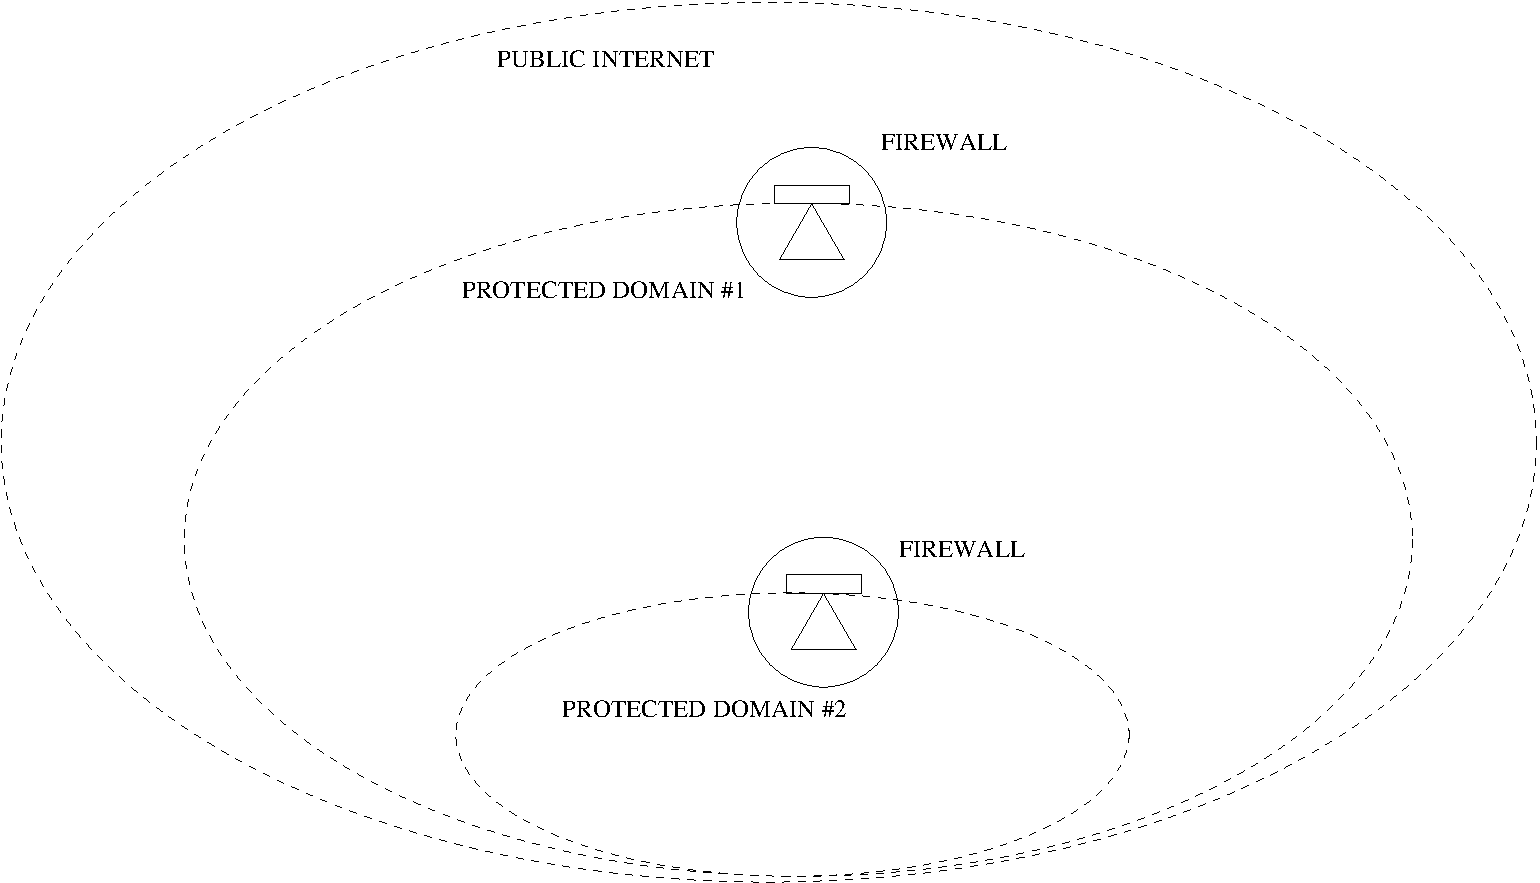
\includegraphics[width=0.5\linewidth]{Figures/Nested_security_domains.pdf}
\else
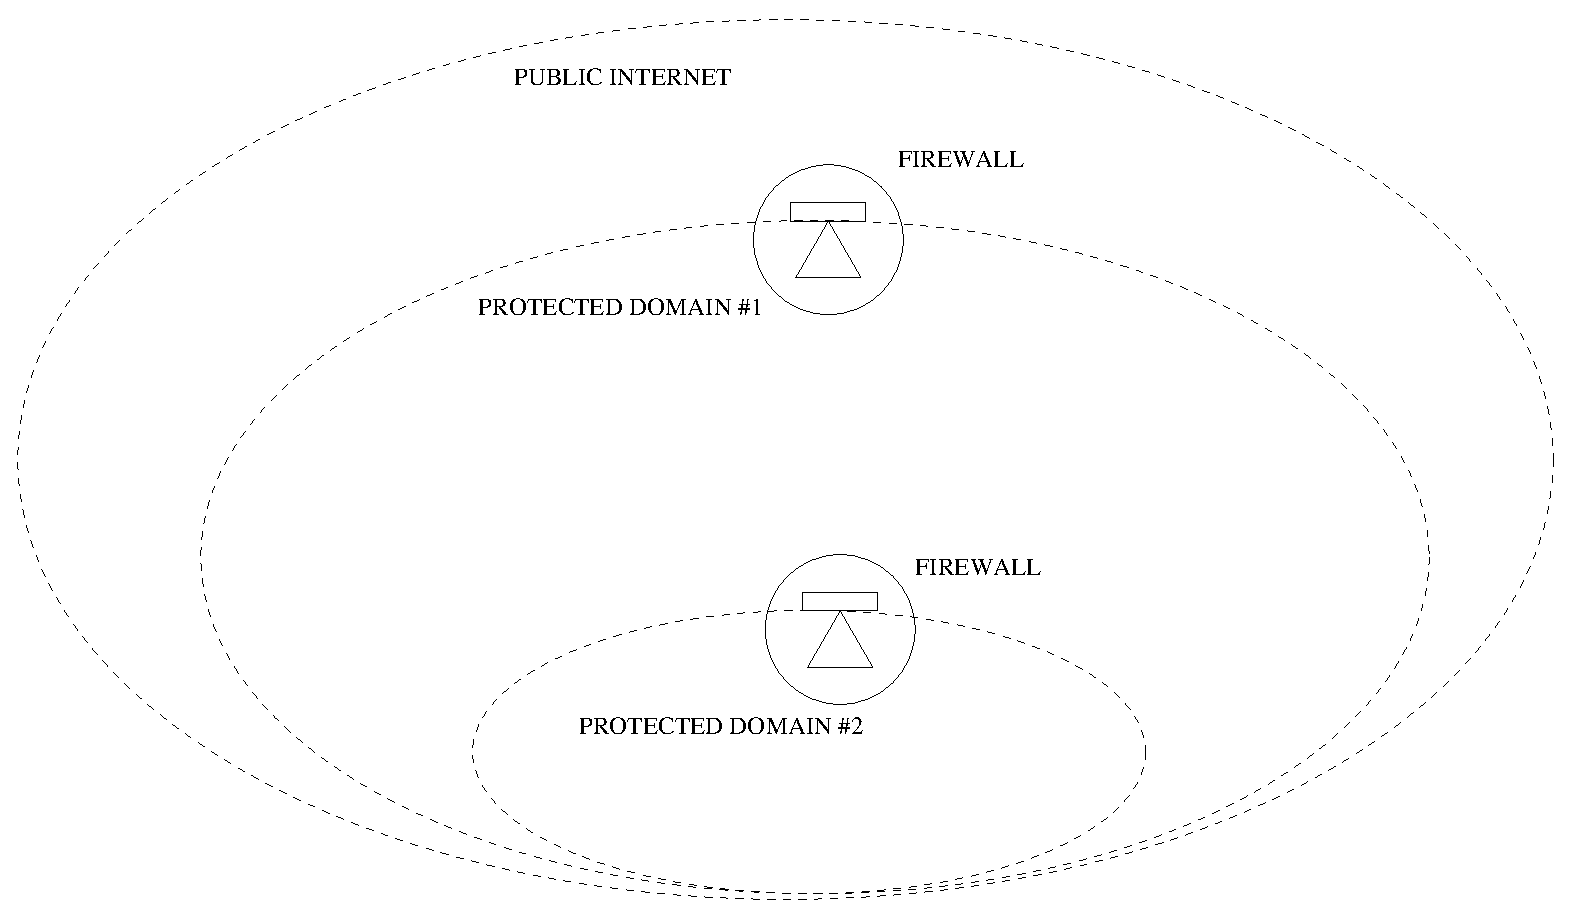
\includegraphics[width=0.5\linewidth]{Figures/Nested_security_domains.eps}
\fi
\caption{Nested security domains.}
\label{fig:Nested_security_domains}
\end{figure}

Another common situation is that an organization wants to expose some information to the internet, for example using web servers.
This web servers need to be placed in a network that can be accessed from the outside.
It is still possible to offer partial protection to this servers using a firewall.
For example, the firewall can be configured to allow only web traffic between the internet and the network of the web servers.
This partially protected network is typically named DMZ (for demilitarized zone).
The organization can keep a network totally protected, as shown in Fig.~\ref{fig:DMZ}.

\begin{figure}
\centering
\ifpdf
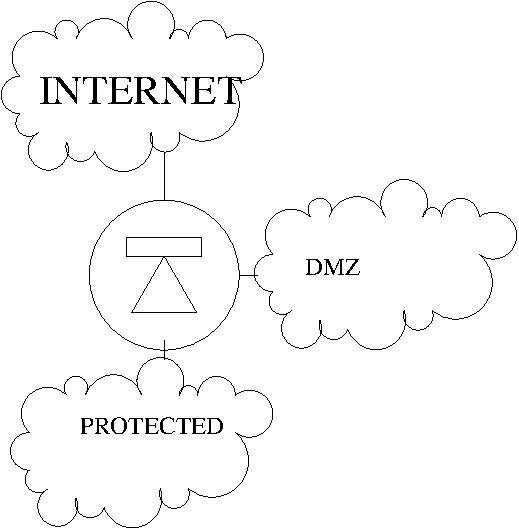
\includegraphics[width=0.5\linewidth]{Figures/DMZ.pdf}
\else
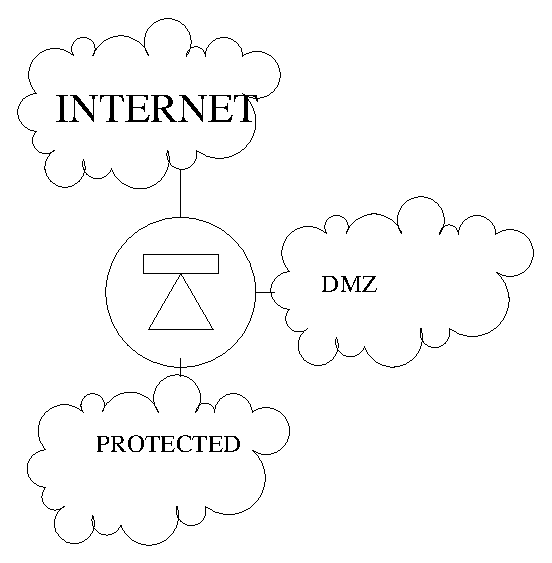
\includegraphics[width=0.5\linewidth]{Figures/DMZ.eps}
\fi
\caption{The firewall separates the public internet, the protected network and a DMZ.}
\label{fig:DMZ}
\end{figure}

There are two possible options to separate the trusted and untrusted domains.
The first one is physical separation, in which the two domains use different hardware.
The second option is logical separation, in which the two domains share some hardware and are logically separated using VLANs or MPLS tags.
Physical separation is considered safer than logical separation.

\subsection{Chain of rules}

There are also to different approaches when configuring a firewall: Permissive access control (reactive) and restrictive access control (proactive).
In the first one, traffic is allowed unless explicitly forbidden.
If a threat is detected, the network administrator adds a new rule to the firewall to protect the network from the threat.
In restrictive access control, the traffic is forbidden unless explicitly allowed.
When a new service requires to send packets through the firewall, the network administrator adds new rules to the firewall to permit the traffic associated to the new service.

A firewall is typically implemented as a chain of rules that are checked one by one until one of the rules matches.
When there is match, the rule has an associated action that can be either allow or deny.
In the case of a restrictive firewall the last rule of the chain denies (rejects) all traffic that does not match any of the previous rules.
In a permissive firewall, the last rules allows any traffic that has not been dropped by any of the previous rules.

The following listing shows an example of a restrictive set of rules:
\begin{lstlisting}
Src             Dst     Protocol        Service            Action
192.168.1.11/32 any     tcp             80                  Allow
192.168.1.0/24  any     any             any                 Drop
any             any     udp             53                  Allow
any             any     any             any                 Drop
\end{lstlisting}

The rules chain applies to a particular interface and a particular direction of traffic.

\subsection{Stateless Firewall}

In its simplest form, a firewall takes decisions based uniquely on the headers of the packet.
This information can include information regarding IP addresses, layer 4 protocol and ports.
For example, a firewall allowing only packets to and from a particular host could be implemented as a stateless firewall.
A firewall that allows all packets that use port 80 as a source or destination port could also be implemented with a stateless firewall.

\subsection{Stateful Firewall}

Consider the previous example of allowing all packets that contain port 80 as either its source or destination port.
This configuration allows the computer in the protected network to browse the web available in servers of the public internet.
A problem with this configuration is that any host of the public internet can access any computer and any port in the protected network by simply using port 80 as its source port.
This configuration gives little protection to the protected network.

An alternative to allow the computers in the protected network to visit web browsers in the public internet while keeping the protected network more secure is to use a stateful firewall.
The stateful firewalls keeps the state of a connection and can take a decision about whether to allow or reject a packet taking into account the history of packets that have traversed the network before.
When a client in the protected network sends a packet to a web server in the public Internet, the firewall stores the addresses and ports of this packet in a database and then will allow the packets that are answering this particular request.
Compared to the stateless firewall that accepted all packets that used port 80, the stateful firewall accept only those packets that are answering a request initiated in the protected network.
Stateful firewalls are much more effective and therefore are the firewalls that we normally use nowadays.

\subsection{Deep Packet Inspection}

Normal firewalls consider only information available in the network layer and the transport layer of the packet.
Deep packet inspection (DPI) is about re-constructing application layer messages and taking decisions based on this information.
A deep packet inspection firewall can differentiate between a web packet and file sharing packet even if they both use exactly the same IP and port information.
A DPI can be much more precise in making decisions thanks to the additional information.
The problem is that the number of applications is very large and is growing continuously.
It is difficult to keep track of all existing applications. 
Furthermore, looking into the application messages and interpreting application information is computationally expensive and consumes CPU time.
Therefore, the packet processing speed is much lower for DPI than it is for normal firewall operation.
Some applications encrypt the information making it more difficult or impossible for the DPI firewall to extract information from the application layer.



